% Options for packages loaded elsewhere
\PassOptionsToPackage{unicode}{hyperref}
\PassOptionsToPackage{hyphens}{url}
%
\documentclass[
]{article}
\usepackage{amsmath,amssymb}
\usepackage{lmodern}
\usepackage{ifxetex,ifluatex}
\ifnum 0\ifxetex 1\fi\ifluatex 1\fi=0 % if pdftex
  \usepackage[T1]{fontenc}
  \usepackage[utf8]{inputenc}
  \usepackage{textcomp} % provide euro and other symbols
\else % if luatex or xetex
  \usepackage{unicode-math}
  \defaultfontfeatures{Scale=MatchLowercase}
  \defaultfontfeatures[\rmfamily]{Ligatures=TeX,Scale=1}
\fi
% Use upquote if available, for straight quotes in verbatim environments
\IfFileExists{upquote.sty}{\usepackage{upquote}}{}
\IfFileExists{microtype.sty}{% use microtype if available
  \usepackage[]{microtype}
  \UseMicrotypeSet[protrusion]{basicmath} % disable protrusion for tt fonts
}{}
\makeatletter
\@ifundefined{KOMAClassName}{% if non-KOMA class
  \IfFileExists{parskip.sty}{%
    \usepackage{parskip}
  }{% else
    \setlength{\parindent}{0pt}
    \setlength{\parskip}{6pt plus 2pt minus 1pt}}
}{% if KOMA class
  \KOMAoptions{parskip=half}}
\makeatother
\usepackage{xcolor}
\IfFileExists{xurl.sty}{\usepackage{xurl}}{} % add URL line breaks if available
\IfFileExists{bookmark.sty}{\usepackage{bookmark}}{\usepackage{hyperref}}
\hypersetup{
  pdftitle={Aflevering 9},
  hidelinks,
  pdfcreator={LaTeX via pandoc}}
\urlstyle{same} % disable monospaced font for URLs
\usepackage[margin=1in]{geometry}
\usepackage{graphicx}
\makeatletter
\def\maxwidth{\ifdim\Gin@nat@width>\linewidth\linewidth\else\Gin@nat@width\fi}
\def\maxheight{\ifdim\Gin@nat@height>\textheight\textheight\else\Gin@nat@height\fi}
\makeatother
% Scale images if necessary, so that they will not overflow the page
% margins by default, and it is still possible to overwrite the defaults
% using explicit options in \includegraphics[width, height, ...]{}
\setkeys{Gin}{width=\maxwidth,height=\maxheight,keepaspectratio}
% Set default figure placement to htbp
\makeatletter
\def\fps@figure{htbp}
\makeatother
\setlength{\emergencystretch}{3em} % prevent overfull lines
\providecommand{\tightlist}{%
  \setlength{\itemsep}{0pt}\setlength{\parskip}{0pt}}
\setcounter{secnumdepth}{-\maxdimen} % remove section numbering
\ifluatex
  \usepackage{selnolig}  % disable illegal ligatures
\fi

\title{Aflevering 9}
\usepackage{etoolbox}
\makeatletter
\providecommand{\subtitle}[1]{% add subtitle to \maketitle
  \apptocmd{\@title}{\par {\large #1 \par}}{}{}
}
\makeatother
\subtitle{Lucas Bagge}
\author{}
\date{\vspace{-2.5em}}

\begin{document}
\maketitle

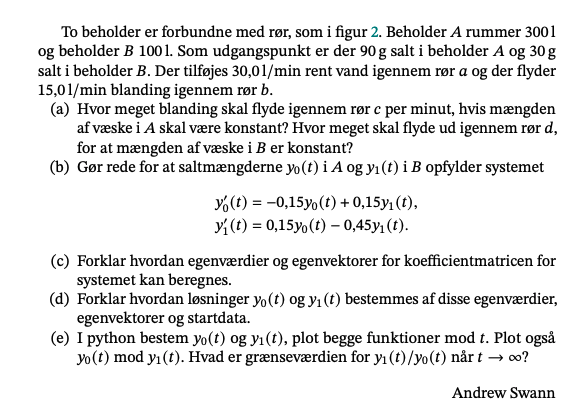
\includegraphics{na-alf-9.png}

\hypertarget{a-definer}{%
\subsection{a) Definer}\label{a-definer}}

I den første del af opgaven skal vi komme frem til hvor meget der kan
flyde igennem rør c per minut og det samme for rør d således at mængden
af væske i respektiv A og B er konstant.

I beholder A er der \textbf{300 L} væske blandet op med \textbf{90g}
salt. Derfor modtager A altså i alt:

\[
65 \ l/min
\]

For at opretholde en konstant mængde væske vil jeg derfor mene at der så
skal flyde \textbf{65 l/min} ud af rør c.~

Den samme ræssonoment bruger jeg til rør d.~Altså at beholder B modtager
65 l/min fra c og der forlader 15 l/min gennem rør b. Der for må der i d
være:

\[
d=65 \ l/min - 15 \ l/min=50 \ l/min
\]

Altså forlader der 50 l/min for at mængden af væske er konstant i
beholder B.

\hypertarget{b}{%
\subsection{b)}\label{b}}

For opgave b skal vi gøre rede for at saltmængderne i A og B kan
opskrives gennem følgende system:

\[
y_0'(t)=\underbrace{-0.15 y_0 (t)}_\textrm{a} + \underbrace{0.15 y_1 (t)}_\textrm{b}
\]

\[
y_1'(t)=\underbrace{0.15 y_0 (t)}_\textrm{c} - \underbrace{0.45 y_1 (t)}_\textrm{d}
\] Her kan vi løse følgende (da vi kender hvad der skal være i hver
beholder)

\[
\frac{a \ l/min}{300 \ l }= 0.15 \ l
\]

\[
a = 300 * 0.15 = -45
\]

a svarer til hvad beholder A mister af salt per minut.

Vi kan bekræfte at b skal være 0.15 ved at kigge på oplysning fra
opgaven da vi kan se at der tilføjes \(15(t_1(t)/100)\) gram salt per
minut. Derfor kan vi sige at det første system er opfyldt med
ovenstående ligning.

Den samme øvelse kan vi gøre med \(y'_1(t)\).

\[
\frac{c \ l/min}{300} = 0.15
\] \[
c = 45
\]

Således passer det med at der skal forlade 45 l/min fra c.~Når det
passer vil vi have at beholder B modtager \(0.15 y_0(t)\) gram salt per
minut.

For at beregne d så skal vi kombiner de to strømme hvor beholder B
mister væske fra, nemlig b og d.~Vi kender b = 15 l/min, mens vi ikke
kender d.~

\[
\frac{15 + d}{100} = 0.45
\]

\[
15+d=45
\]

\[
d = 30
\]

Altså vil det sige at der flyder 30 l/min salt ud af rør d.

Når det gælder så vil saltmængderne i \(y_0\) og \(y_1\) være opfyldt.

\hypertarget{c}{%
\subsection{c)}\label{c}}

Her skal vi forklare hvordan egenværdier og egenvektorer for
koefficientmatricen kan beregnes.

Vi kan starte med at opskrive systemet op i vektor notation som er vist
ved ligning 22.2 i note sættet:

\[
A = \begin{bmatrix}
-0.15 &  0.15 \\
 0.15 & -0.45 
\end{bmatrix}
\]

Hvor begyndelseværdier er angivet ved mængden af salt:

\[
y(0)=
\begin{bmatrix}
90 \\
30
\end{bmatrix}
\] Egenværiderne og egenvektor kan beregnes ved at regne det
karakteristik polynomium og herved check om A er diagonaliserbar.

opskriv det karakteristik polynomium

\[
det  =
\begin{bmatrix}
-0.15 - \lambda & 0.15 \\
0.15 & -0.45-\lambda
\end{bmatrix}
= \lambda^2+0.6\lambda+0.045
\] Som har rødderne:

\[
\frac{-0.6+-\sqrt{0.6^2-4*1*0.045}}{2*1}
\] \[
\text{med egenværdierne; } \ -0.512, \ -0.089
\]

Matricen er en 2 x 2 matrix og vi har to forskellig rødde så A er
diagonaliserbar.

Hvorefter vi kan beregne egenvektor for hver egenværdier. Her benytter
jeg mig af et cas værkstøj til disse udregninger.

Her får jeg en egenvektor til \(v_0=(2.41,1)\) og \(v_1=(-0.4142,1)\)

Hermed har jeg udfra det karakteristiske polynomium og det faktum at A
er diagonaliserbar fundet frem til egenværdierne og egenvektorerne.

\hypertarget{d}{%
\subsection{d)}\label{d}}

Her skal vi nu bestemme en løsning.

Løsnigen kan beregnes ved at opsætte et ligning system som følger
proposition 22.2.

Den manuelle beregning vil jeg foretage her og i opgave e skal de regnes
i python.

For en løsning benytter vi os af proposition 22.2:

\[
y(t) = c_0 \begin{bmatrix} 2.41 \\ 1\end{bmatrix}e^{-0.512 t} +c_1
\begin{bmatrix} -0.4141 \\ 1\end{bmatrix}e^{-0.089 t}
\] Her kan vi bestemme konstanterne c0 go c1 ud fra begyndelsesdata. Ved
t =0 har vi

\[
y(0)=c_0 \begin{bmatrix} 2.41\\ 1\end{bmatrix}+c_1 \begin{bmatrix} -0.4141\\1 \end{bmatrix}=\begin{bmatrix} 90\\30\end{bmatrix}
\]

Som har løsningen \(c_1=36.267\) og \(c_2=-6.267\)

\hypertarget{e}{%
\subsection{e)}\label{e}}

\end{document}
